\documentclass{beamer}

\usefonttheme{professionalfonts} % using non standard fonts for beamer
\usefonttheme{serif} % default family is serif

\usepackage{hyperref}

%\usepackage{minted}

\usepackage{animate}

\usepackage{graphicx}

\def\Put(#1,#2)#3{\leavevmode\makebox(0,0){\put(#1,#2){#3}}}

\usepackage{color}

\usepackage{tikz}

\usepackage{amssymb}

\usepackage{enumerate}


\newcommand\blfootnote[1]{%

  \begingroup

  \renewcommand\thefootnote{}\footnote{#1}%

  \addtocounter{footnote}{-1}%

  \endgroup

}

\makeatletter

%%%%%%%%%%%%%%%%%%%%%%%%%%%%%% Textclass specific LaTeX commands.

 % this default might be overridden by plain title style

 \newcommand\makebeamertitle{\frame{\maketitle}}%

 % (ERT) argument for the TOC

 \AtBeginDocument{%

   \let\origtableofcontents=\tableofcontents

   \def\tableofcontents{\@ifnextchar[{\origtableofcontents}{\gobbletableofcontents}}

   \def\gobbletableofcontents#1{\origtableofcontents}

 }

%%%%%%%%%%%%%%%%%%%%%%%%%%%%%% User specified LaTeX commands.

\usetheme{Malmoe}

% or ...

\useoutertheme{infolines}

\addtobeamertemplate{headline}{}{\vskip2pt}



\setbeamercovered{transparent}

% or whatever (possibly just delete it)

\makeatother

\begin{document}
\title[DCEL report]{RIDIR Report}
\author[AC]{Andres Calderon}
\institute[Fall'19]{University of California, Riverside}
\makebeamertitle
\newif\iflattersubsect

\AtBeginSection[] {
    \begin{frame}<beamer>
    \frametitle{Outline} 
    \tableofcontents[currentsection]  
    \end{frame}
    \lattersubsectfalse
}

\AtBeginSubsection[] {
    \begin{frame}<beamer>
    \frametitle{Outline} 
    \tableofcontents[currentsubsection]  
    \end{frame}
}

\begin{frame}{OGC specification}
    \begin{itemize}
        \item OpenGIS Implementation Standard for Geographic information - Simple feature access\footnote{http://www.opengeospatial.org/standards/sfa}
        \begin{itemize}
            \item Section 6.1.11 Polygons:  Clarify format for polygons with holes. \\
            i.e. POLYGON (\\
            \hspace{10pt}( exterior ring ), ( interior rings )*\\
            )
            \item Section 6.1.14 Multipolygons:  Clarify the format for multipolygons. \\
            i.e. MULTIPOLYGON (\\
            \hspace{10pt}(( polygon 1 )),\\
            \hspace{10pt}(( polygon 2 )),\\
            \hspace{10pt}(( polygon n ))*\\
            )
        \end{itemize}
    \end{itemize}
\end{frame}

\begin{frame}{OGC specification}
    \begin{itemize}
        \item OGC specification also provides methods to get number of holes and geometries and check if a feature is simple and valid.
        \item JTS library (GeoSpark) implements the OGC implementation.
        \item I have coded a simple \textbf{GeometryChecker} routine to obtaing info about the input layers.
    \end{itemize}
\end{frame}

\begin{frame}{Dealing with holes}
    \begin{itemize}
        \item With the methods provided by JTS it was easier to track the holes and which polygon their belongs to and adjust the DCEL accordingly.
        \item First tried with demo polygons in sequential and parallel approaches.  Then tested with a bigger dataset (California districts).
        \item The output is consistent with the expected results.
    \end{itemize}
\end{frame}

\begin{frame}{Validation - Demo sequential}
    \centering 
    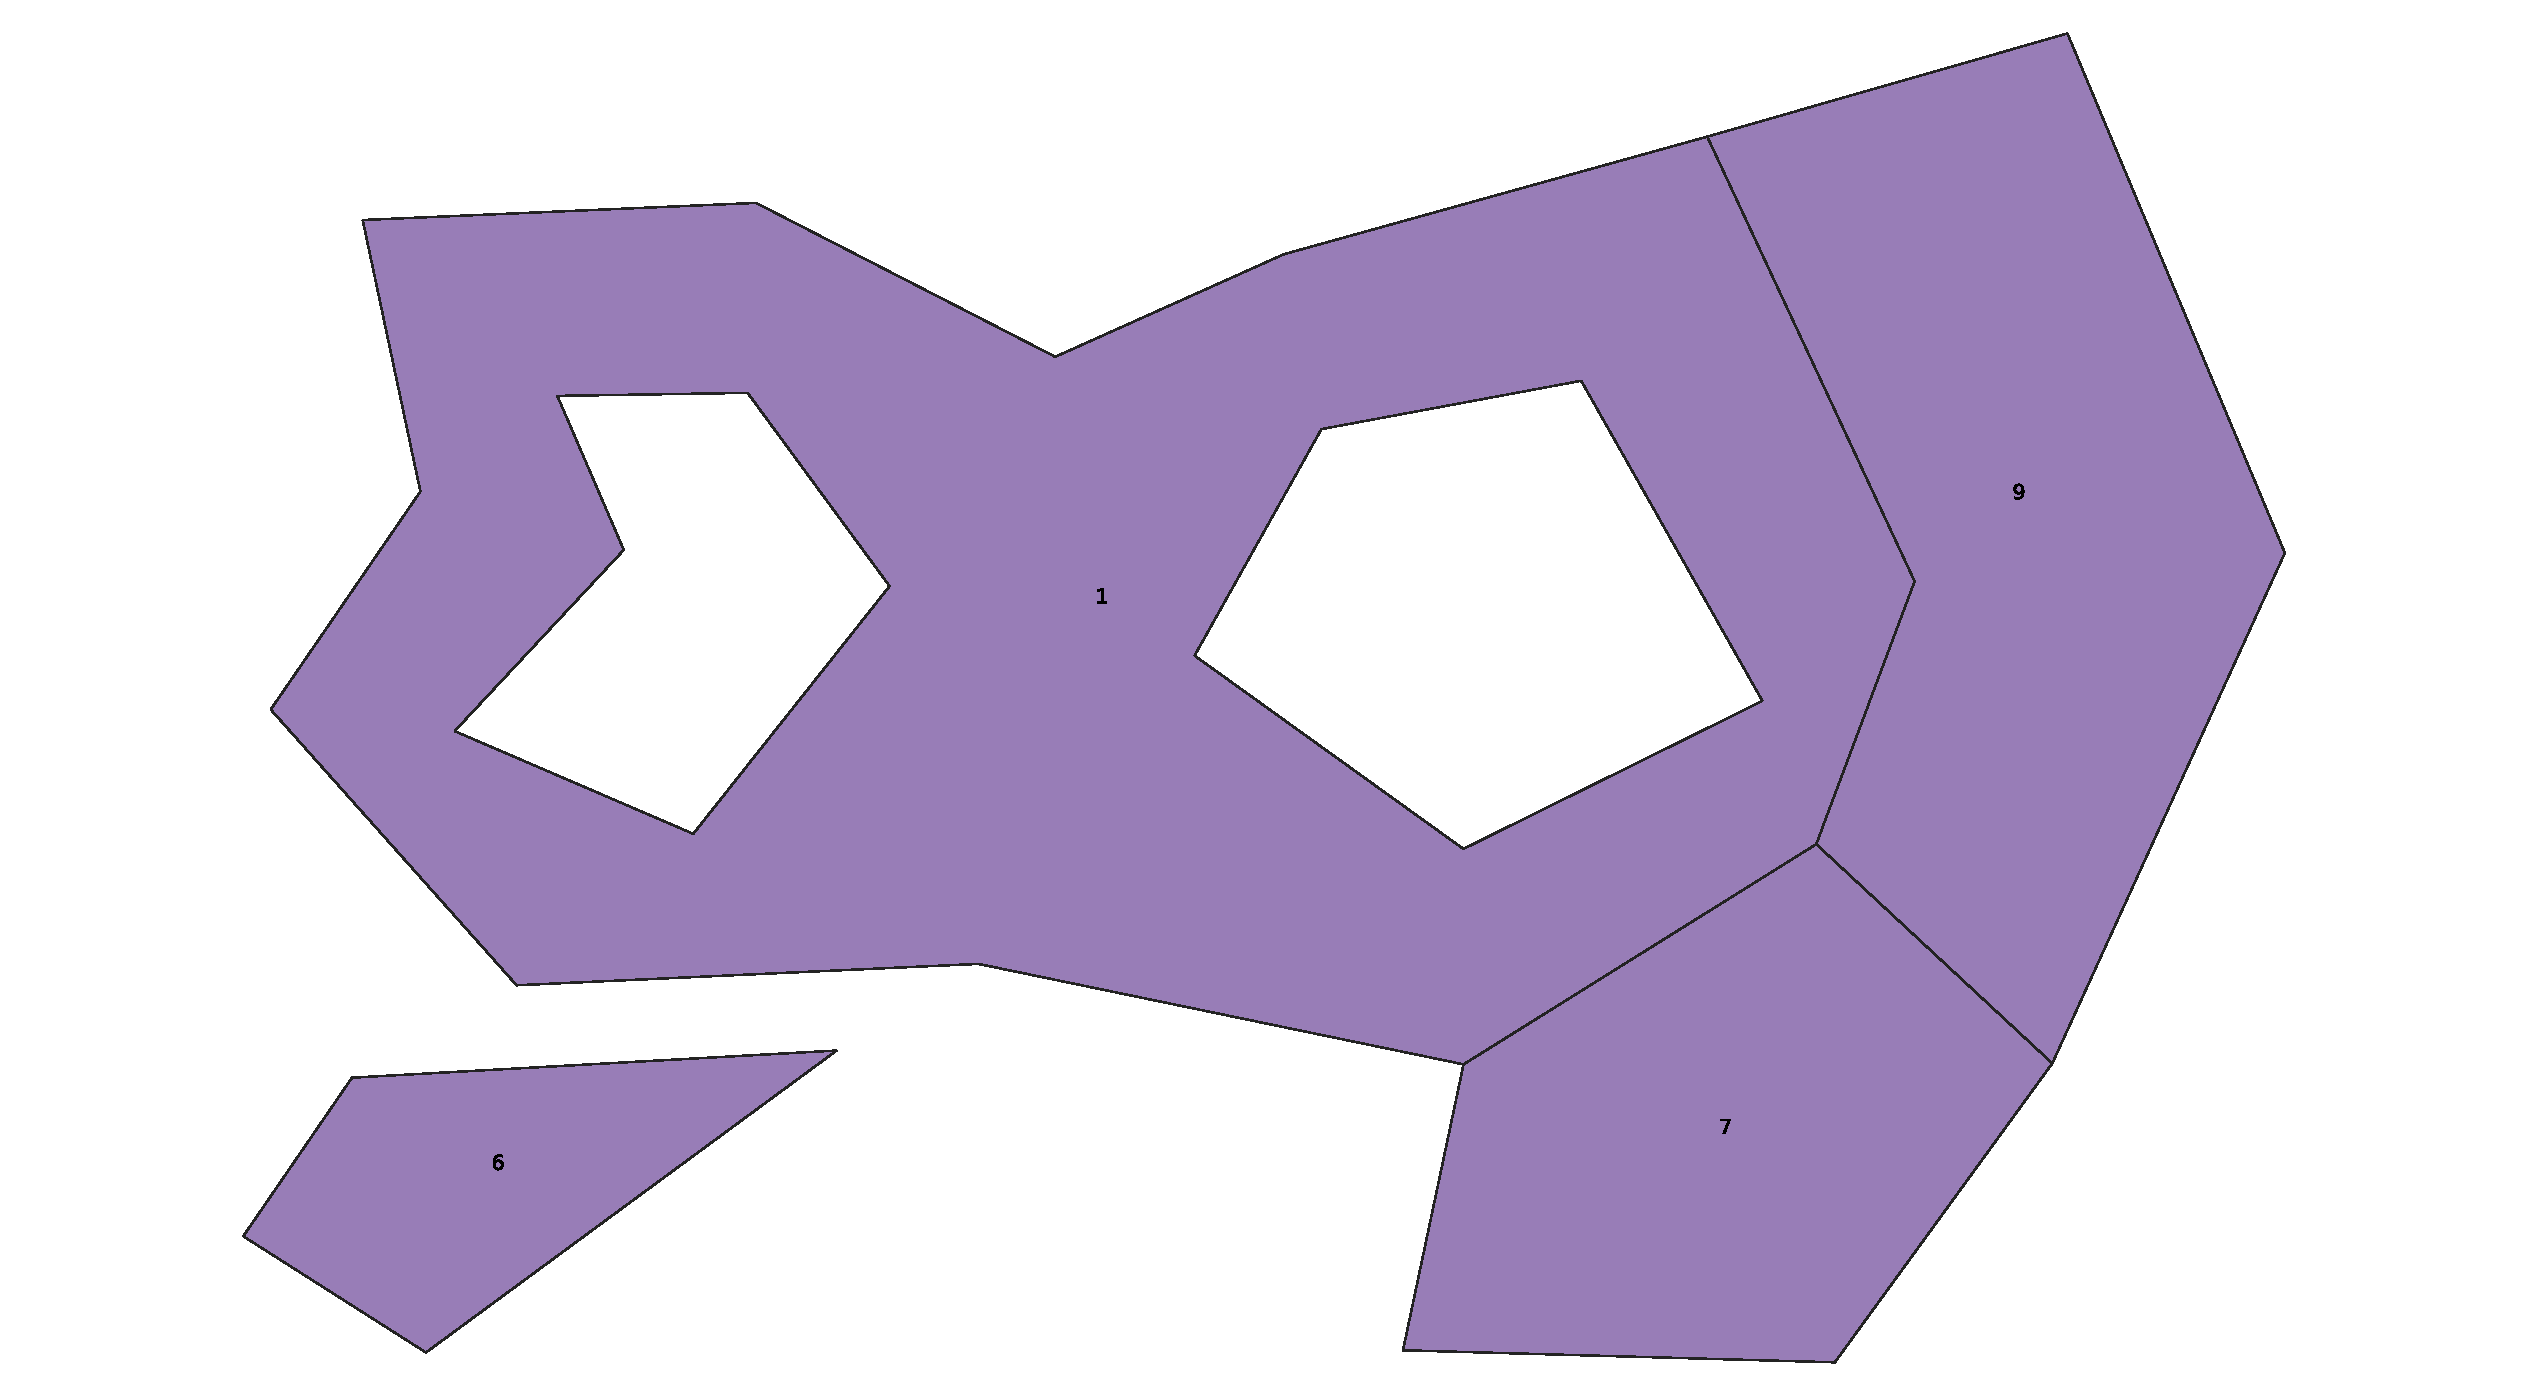
\includegraphics[width=0.9\linewidth]{figures/Demo_sequential} 
\end{frame}

\begin{frame}{Validation - Demo parallel}
    \centering 
    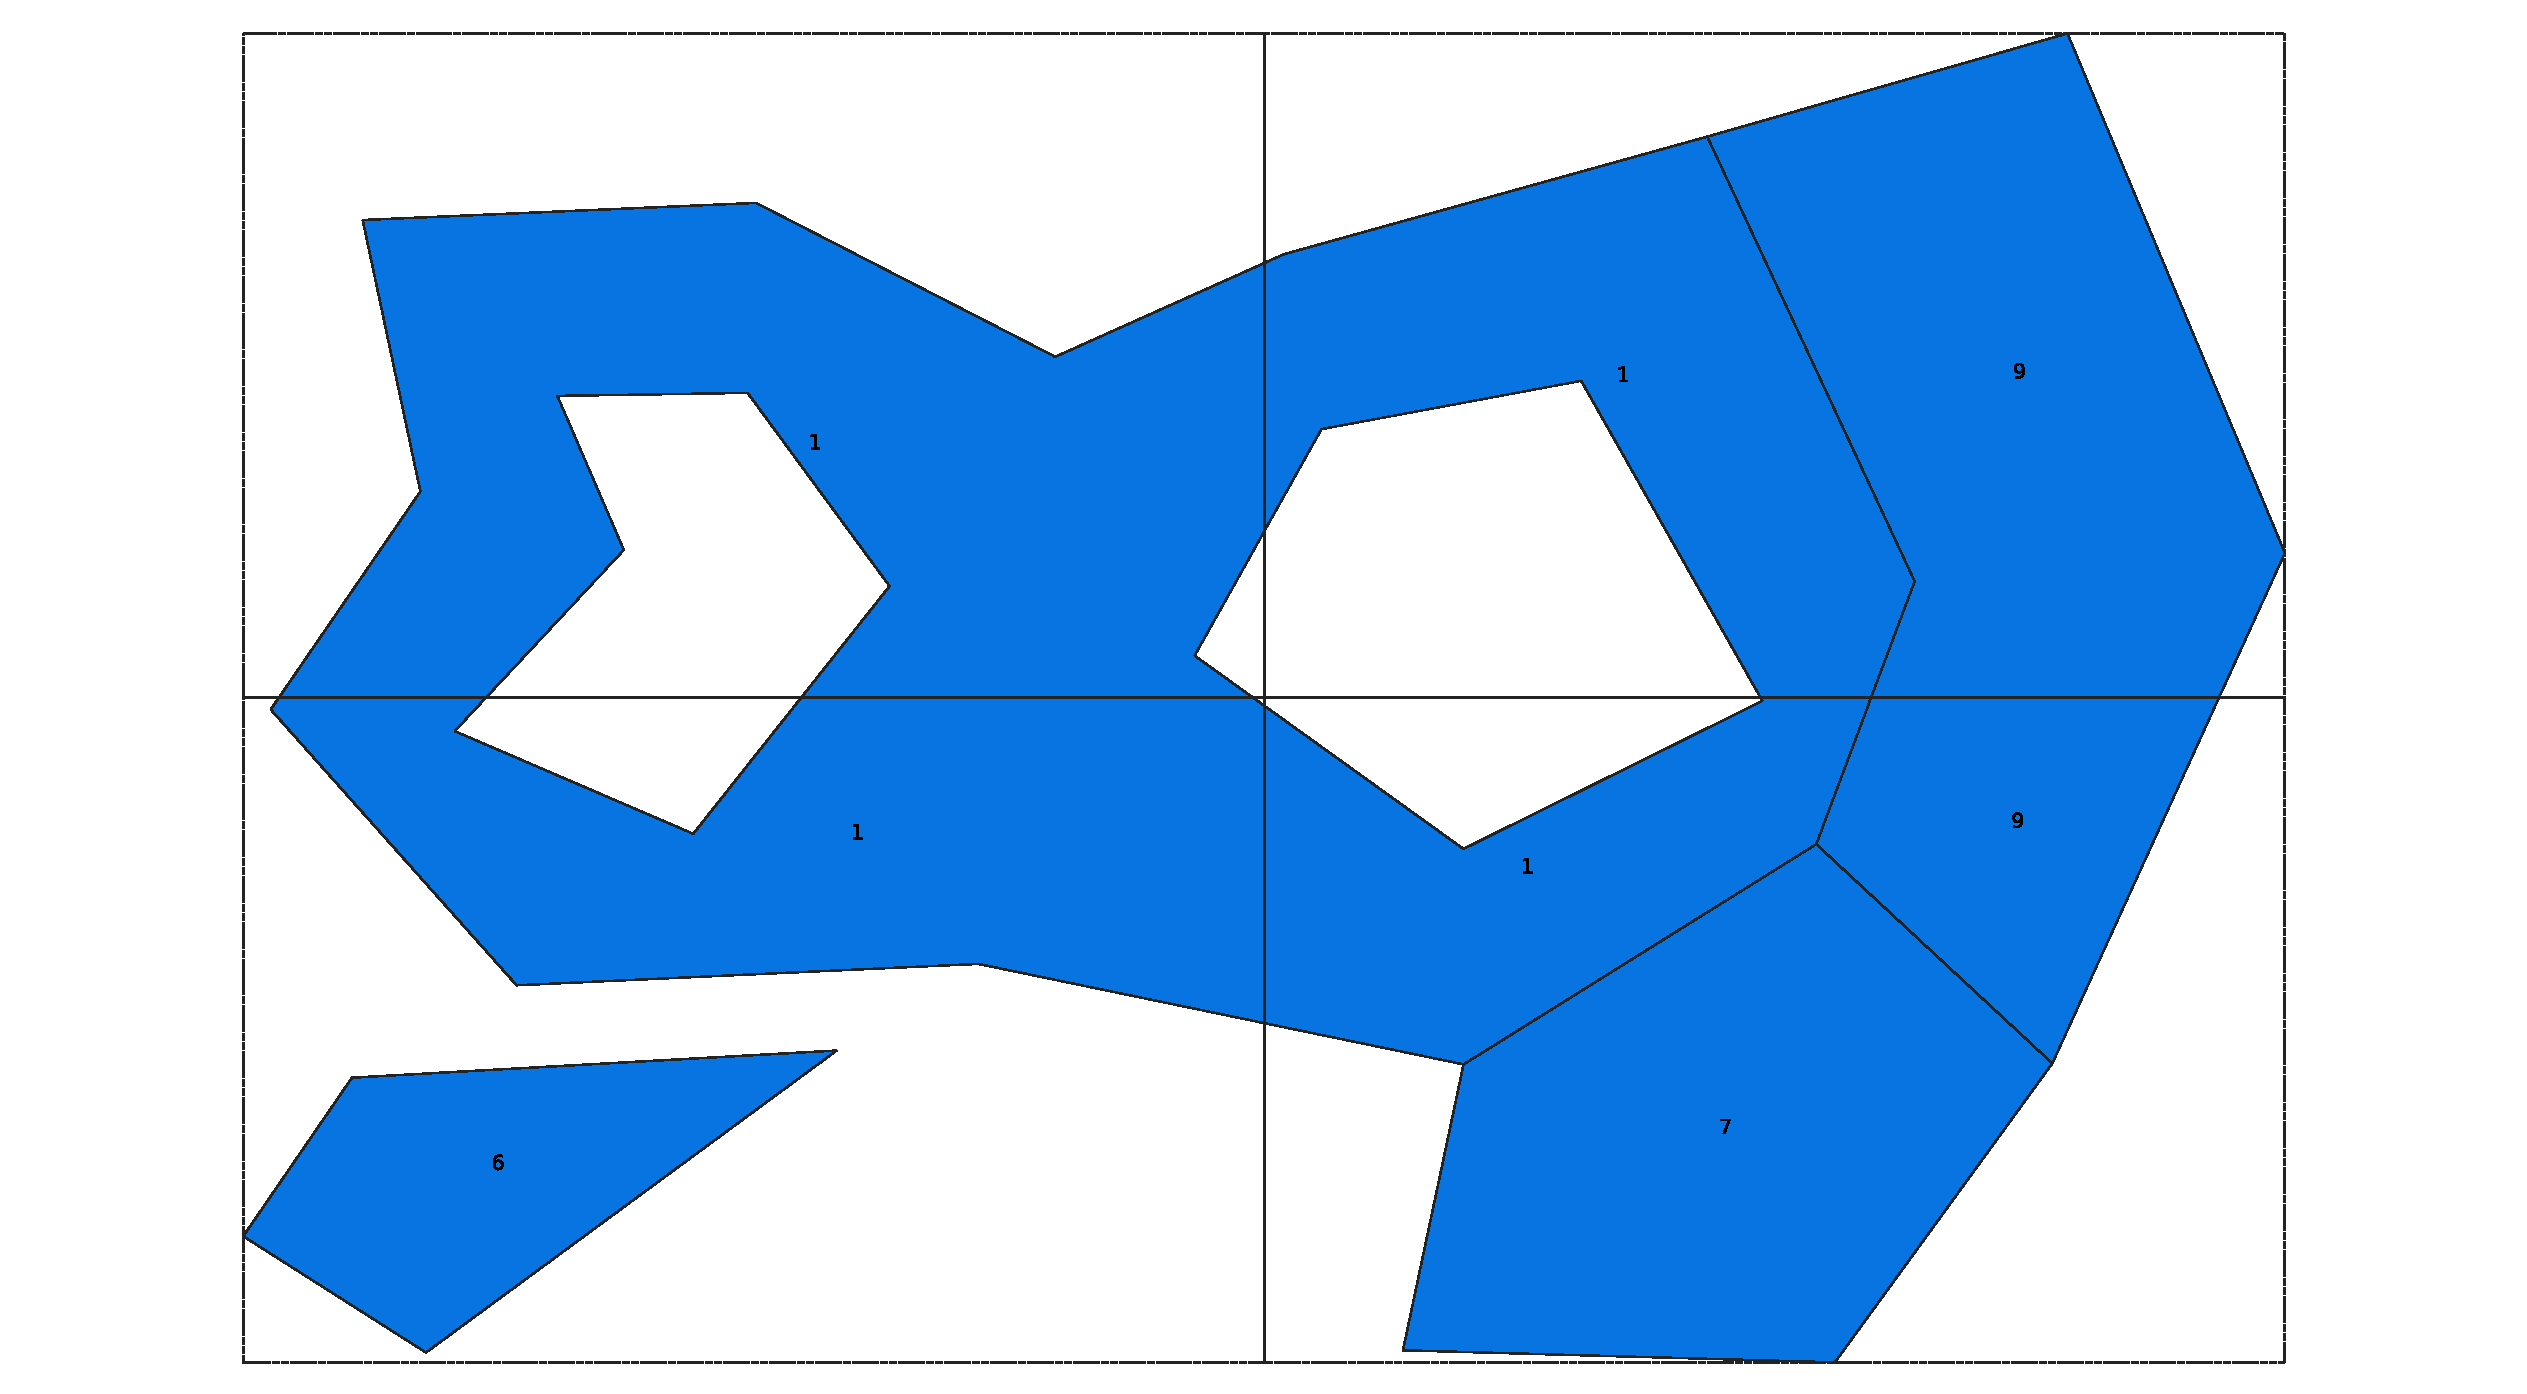
\includegraphics[width=0.9\linewidth]{figures/Demo_parallel} 
\end{frame}

\begin{frame}{Validation - CA\_sample parallel}
    \centering 
    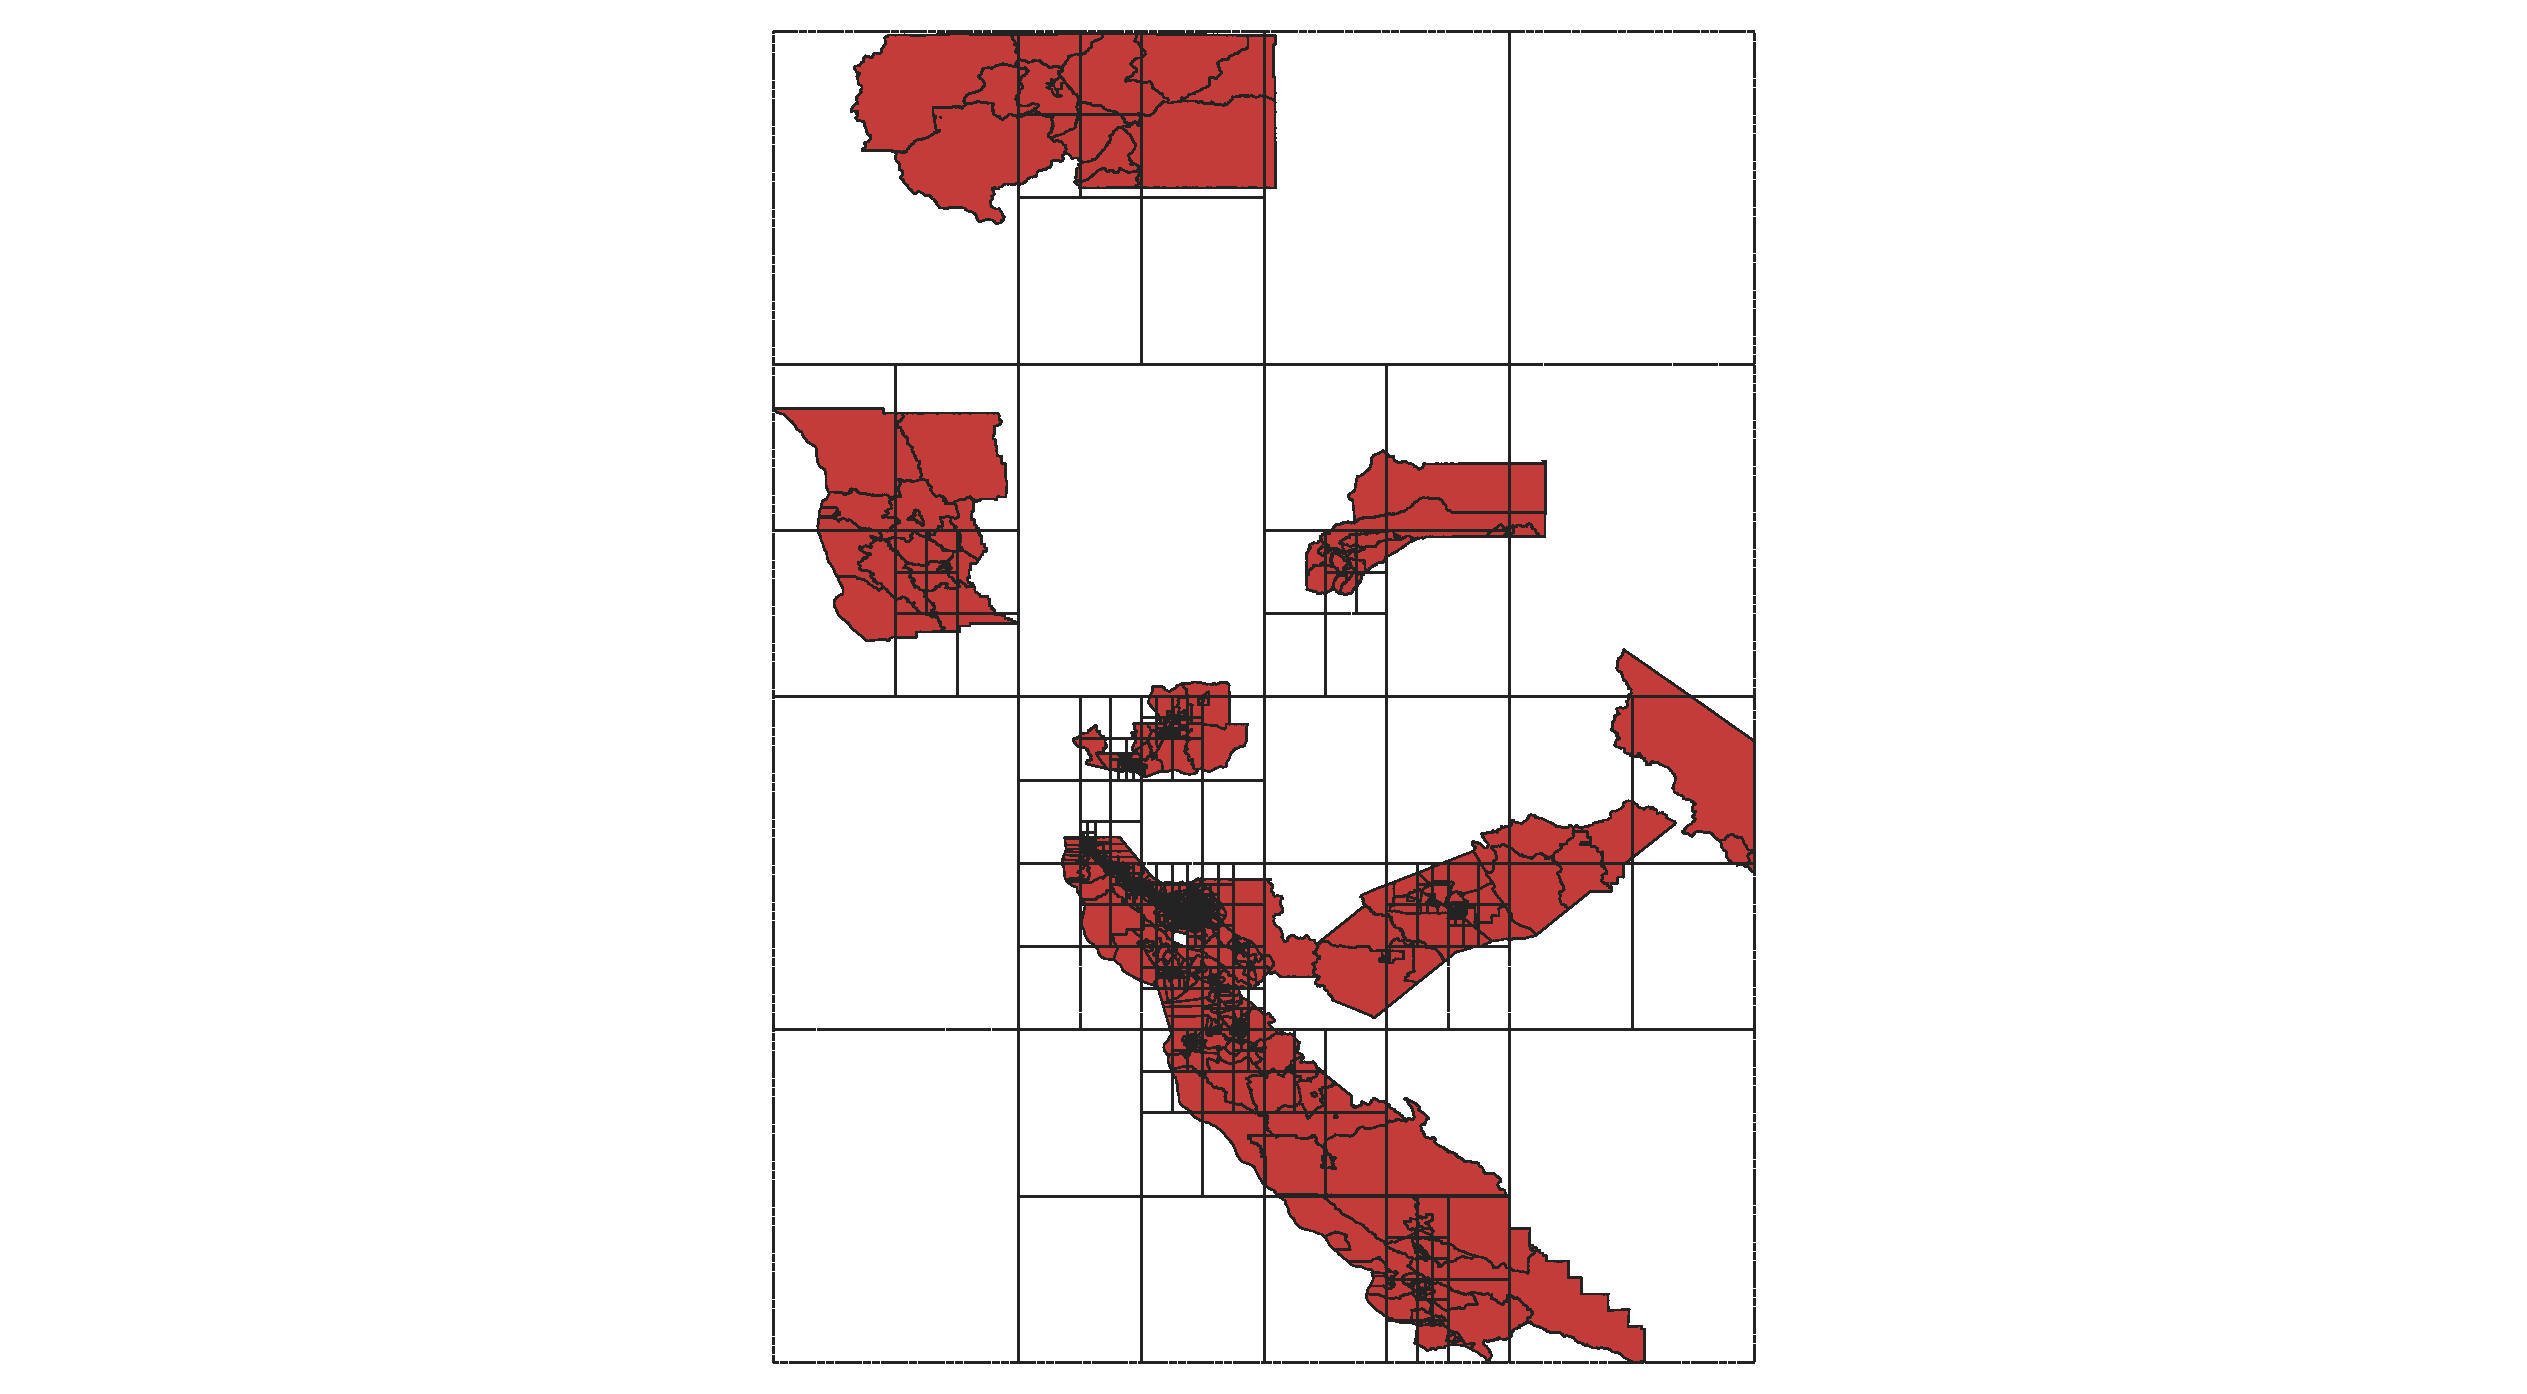
\includegraphics[width=\linewidth]{figures/CA_test} 
\end{frame}

\begin{frame}{What is next?}
    \begin{itemize}
        \item Fix bug during reading of WKT features.
        \item Check support for multipolygons.
        \item Integrate changes in merged DCEL.
        \item Test with bigger datasets.
    \end{itemize}
\end{frame}

\end{document}
